
%% bare_conf_compsoc.tex
%% V1.4b
%% 2015/08/26
%% by Michael Shell
%% See:
%% http://www.michaelshell.org/
%% for current contact information.
%%
%% This is a skeleton file demonstrating the use of IEEEtran.cls
%% (requires IEEEtran.cls version 1.8b or later) with an IEEE Computer
%% Society conference paper.
%%
%% Support sites:
%% http://www.michaelshell.org/tex/ieeetran/
%% http://www.ctan.org/pkg/ieeetran
%% and
%% http://www.ieee.org/

%%*************************************************************************
%% Legal Notice:
%% This code is offered as-is without any warranty either expressed or
%% implied; without even the implied warranty of MERCHANTABILITY or
%% FITNESS FOR A PARTICULAR PURPOSE! 
%% User assumes all risk.
%% In no event shall the IEEE or any contributor to this code be liable for
%% any damages or losses, including, but not limited to, incidental,
%% consequential, or any other damages, resulting from the use or misuse
%% of any information contained here.
%%
%% All comments are the opinions of their respective authors and are not
%% necessarily endorsed by the IEEE.
%%
%% This work is distributed under the LaTeX Project Public License (LPPL)
%% ( http://www.latex-project.org/ ) version 1.3, and may be freely used,
%% distributed and modified. A copy of the LPPL, version 1.3, is included
%% in the base LaTeX documentation of all distributions of LaTeX released
%% 2003/12/01 or later.
%% Retain all contribution notices and credits.
%% ** Modified files should be clearly indicated as such, including  **
%% ** renaming them and changing author support contact information. **
%%*************************************************************************


% *** Authors should verify (and, if needed, correct) their LaTeX system  ***
% *** with the testflow diagnostic prior to trusting their LaTeX platform ***
% *** with production work. The IEEE's font choices and paper sizes can   ***
% *** trigger bugs that do not appear when using other class files.       ***                          ***
% The testflow support page is at:
% http://www.michaelshell.org/tex/testflow/



\documentclass[conference,compsoc]{IEEEtran}
% Some/most Computer Society conferences require the compsoc mode option,
% but others may want the standard conference format.
%
% If IEEEtran.cls has not been installed into the LaTeX system files,
% manually specify the path to it like:
% \documentclass[conference,compsoc]{../sty/IEEEtran}


\usepackage{graphicx}
\graphicspath{{plots/}}


% Some very useful LaTeX packages include:
% (uncomment the ones you want to load)


% *** MISC UTILITY PACKAGES ***
%
%\usepackage{ifpdf}
% Heiko Oberdiek's ifpdf.sty is very useful if you need conditional
% compilation based on whether the output is pdf or dvi.
% usage:
% \ifpdf
%   % pdf code
% \else
%   % dvi code
% \fi
% The latest version of ifpdf.sty can be obtained from:
% http://www.ctan.org/pkg/ifpdf
% Also, note that IEEEtran.cls V1.7 and later provides a builtin
% \ifCLASSINFOpdf conditional that works the same way.
% When switching from latex to pdflatex and vice-versa, the compiler may
% have to be run twice to clear warning/error messages.






% *** CITATION PACKAGES ***
%
\ifCLASSOPTIONcompsoc
  % IEEE Computer Society needs nocompress option
  % requires cite.sty v4.0 or later (November 2003)
  \usepackage[nocompress]{cite}
\else
  % normal IEEE
  \usepackage{cite}
\fi
% cite.sty was written by Donald Arseneau
% V1.6 and later of IEEEtran pre-defines the format of the cite.sty package
% \cite{} output to follow that of the IEEE. Loading the cite package will
% result in citation numbers being automatically sorted and properly
% "compressed/ranged". e.g., [1], [9], [2], [7], [5], [6] without using
% cite.sty will become [1], [2], [5]--[7], [9] using cite.sty. cite.sty's
% \cite will automatically add leading space, if needed. Use cite.sty's
% noadjust option (cite.sty V3.8 and later) if you want to turn this off
% such as if a citation ever needs to be enclosed in parenthesis.
% cite.sty is already installed on most LaTeX systems. Be sure and use
% version 5.0 (2009-03-20) and later if using hyperref.sty.
% The latest version can be obtained at:
% http://www.ctan.org/pkg/cite
% The documentation is contained in the cite.sty file itself.
%
% Note that some packages require special options to format as the Computer
% Society requires. In particular, Computer Society  papers do not use
% compressed citation ranges as is done in typical IEEE papers
% (e.g., [1]-[4]). Instead, they list every citation separately in order
% (e.g., [1], [2], [3], [4]). To get the latter we need to load the cite
% package with the nocompress option which is supported by cite.sty v4.0
% and later.





% *** GRAPHICS RELATED PACKAGES ***
%
\ifCLASSINFOpdf
  % \usepackage[pdftex]{graphicx}
  % declare the path(s) where your graphic files are
  % \graphicspath{{../pdf/}{../jpeg/}}
  % and their extensions so you won't have to specify these with
  % every instance of \includegraphics
  % \DeclareGraphicsExtensions{.pdf,.jpeg,.png}
\else
  % or other class option (dvipsone, dvipdf, if not using dvips). graphicx
  % will default to the driver specified in the system graphics.cfg if no
  % driver is specified.
  % \usepackage[dvips]{graphicx}
  % declare the path(s) where your graphic files are
  % \graphicspath{{../eps/}}
  % and their extensions so you won't have to specify these with
  % every instance of \includegraphics
  % \DeclareGraphicsExtensions{.eps}
\fi
% graphicx was written by David Carlisle and Sebastian Rahtz. It is
% required if you want graphics, photos, etc. graphicx.sty is already
% installed on most LaTeX systems. The latest version and documentation
% can be obtained at: 
% http://www.ctan.org/pkg/graphicx
% Another good source of documentation is "Using Imported Graphics in
% LaTeX2e" by Keith Reckdahl which can be found at:
% http://www.ctan.org/pkg/epslatex
%
% latex, and pdflatex in dvi mode, support graphics in encapsulated
% postscript (.eps) format. pdflatex in pdf mode supports graphics
% in .pdf, .jpeg, .png and .mps (metapost) formats. Users should ensure
% that all non-photo figures use a vector format (.eps, .pdf, .mps) and
% not a bitmapped formats (.jpeg, .png). The IEEE frowns on bitmapped formats
% which can result in "jaggedy"/blurry rendering of lines and letters as
% well as large increases in file sizes.
%
% You can find documentation about the pdfTeX application at:
% http://www.tug.org/applications/pdftex





% *** MATH PACKAGES ***
%
%\usepackage{amsmath}
% A popular package from the American Mathematical Society that provides
% many useful and powerful commands for dealing with mathematics.
%
% Note that the amsmath package sets \interdisplaylinepenalty to 10000
% thus preventing page breaks from occurring within multiline equations. Use:
%\interdisplaylinepenalty=2500
% after loading amsmath to restore such page breaks as IEEEtran.cls normally
% does. amsmath.sty is already installed on most LaTeX systems. The latest
% version and documentation can be obtained at:
% http://www.ctan.org/pkg/amsmath





% *** SPECIALIZED LIST PACKAGES ***
%
%\usepackage{algorithmic}
% algorithmic.sty was written by Peter Williams and Rogerio Brito.
% This package provides an algorithmic environment fo describing algorithms.
% You can use the algorithmic environment in-text or within a figure
% environment to provide for a floating algorithm. Do NOT use the algorithm
% floating environment provided by algorithm.sty (by the same authors) or
% algorithm2e.sty (by Christophe Fiorio) as the IEEE does not use dedicated
% algorithm float types and packages that provide these will not provide
% correct IEEE style captions. The latest version and documentation of
% algorithmic.sty can be obtained at:
% http://www.ctan.org/pkg/algorithms
% Also of interest may be the (relatively newer and more customizable)
% algorithmicx.sty package by Szasz Janos:
% http://www.ctan.org/pkg/algorithmicx




% *** ALIGNMENT PACKAGES ***
%
%\usepackage{array}
% Frank Mittelbach's and David Carlisle's array.sty patches and improves
% the standard LaTeX2e array and tabular environments to provide better
% appearance and additional user controls. As the default LaTeX2e table
% generation code is lacking to the point of almost being broken with
% respect to the quality of the end results, all users are strongly
% advised to use an enhanced (at the very least that provided by array.sty)
% set of table tools. array.sty is already installed on most systems. The
% latest version and documentation can be obtained at:
% http://www.ctan.org/pkg/array


% IEEEtran contains the IEEEeqnarray family of commands that can be used to
% generate multiline equations as well as matrices, tables, etc., of high
% quality.




% *** SUBFIGURE PACKAGES ***
%\ifCLASSOPTIONcompsoc
%  \usepackage[caption=false,font=footnotesize,labelfont=sf,textfont=sf]{subfig}
%\else
%  \usepackage[caption=false,font=footnotesize]{subfig}
%\fi
% subfig.sty, written by Steven Douglas Cochran, is the modern replacement
% for subfigure.sty, the latter of which is no longer maintained and is
% incompatible with some LaTeX packages including fixltx2e. However,
% subfig.sty requires and automatically loads Axel Sommerfeldt's caption.sty
% which will override IEEEtran.cls' handling of captions and this will result
% in non-IEEE style figure/table captions. To prevent this problem, be sure
% and invoke subfig.sty's "caption=false" package option (available since
% subfig.sty version 1.3, 2005/06/28) as this is will preserve IEEEtran.cls
% handling of captions.
% Note that the Computer Society format requires a sans serif font rather
% than the serif font used in traditional IEEE formatting and thus the need
% to invoke different subfig.sty package options depending on whether
% compsoc mode has been enabled.
%
% The latest version and documentation of subfig.sty can be obtained at:
% http://www.ctan.org/pkg/subfig




% *** FLOAT PACKAGES ***
%
%\usepackage{fixltx2e}
% fixltx2e, the successor to the earlier fix2col.sty, was written by
% Frank Mittelbach and David Carlisle. This package corrects a few problems
% in the LaTeX2e kernel, the most notable of which is that in current
% LaTeX2e releases, the ordering of single and double column floats is not
% guaranteed to be preserved. Thus, an unpatched LaTeX2e can allow a
% single column figure to be placed prior to an earlier double column
% figure.
% Be aware that LaTeX2e kernels dated 2015 and later have fixltx2e.sty's
% corrections already built into the system in which case a warning will
% be issued if an attempt is made to load fixltx2e.sty as it is no longer
% needed.
% The latest version and documentation can be found at:
% http://www.ctan.org/pkg/fixltx2e


%\usepackage{stfloats}
% stfloats.sty was written by Sigitas Tolusis. This package gives LaTeX2e
% the ability to do double column floats at the bottom of the page as well
% as the top. (e.g., "\begin{figure*}[!b]" is not normally possible in
% LaTeX2e). It also provides a command:
%\fnbelowfloat
% to enable the placement of footnotes below bottom floats (the standard
% LaTeX2e kernel puts them above bottom floats). This is an invasive package
% which rewrites many portions of the LaTeX2e float routines. It may not work
% with other packages that modify the LaTeX2e float routines. The latest
% version and documentation can be obtained at:
% http://www.ctan.org/pkg/stfloats
% Do not use the stfloats baselinefloat ability as the IEEE does not allow
% \baselineskip to stretch. Authors submitting work to the IEEE should note
% that the IEEE rarely uses double column equations and that authors should try
% to avoid such use. Do not be tempted to use the cuted.sty or midfloat.sty
% packages (also by Sigitas Tolusis) as the IEEE does not format its papers in
% such ways.
% Do not attempt to use stfloats with fixltx2e as they are incompatible.
% Instead, use Morten Hogholm'a dblfloatfix which combines the features
% of both fixltx2e and stfloats:
%
% \usepackage{dblfloatfix}
% The latest version can be found at:
% http://www.ctan.org/pkg/dblfloatfix




% *** PDF, URL AND HYPERLINK PACKAGES ***
%
%\usepackage{url}
% url.sty was written by Donald Arseneau. It provides better support for
% handling and breaking URLs. url.sty is already installed on most LaTeX
% systems. The latest version and documentation can be obtained at:
% http://www.ctan.org/pkg/url
% Basically, \url{my_url_here}.




% *** Do not adjust lengths that control margins, column widths, etc. ***
% *** Do not use packages that alter fonts (such as pslatex).         ***
% There should be no need to do such things with IEEEtran.cls V1.6 and later.
% (Unless specifically asked to do so by the journal or conference you plan
% to submit to, of course. )


% correct bad hyphenation here
\hyphenation{op-tical net-works semi-conduc-tor}

\usepackage{hyperref}
\usepackage{tabularx}
\begin{document}
%
% paper title
% Titles are generally capitalized except for words such as a, an, and, as,
% at, but, by, for, in, nor, of, on, or, the, to and up, which are usually
% not capitalized unless they are the first or last word of the title.
% Linebreaks \\ can be used within to get better formatting as desired.
% Do not put math or special symbols in the title.
\title{Scientific Co-authorship Network at IITM}




% conference papers do not typically use \thanks and this command
% is locked out in conference mode. If really needed, such as for
% the acknowledgment of grants, issue a \IEEEoverridecommandlockouts
% after \documentclass

% for over three affiliations, or if they all won't fit within the width
% of the page (and note that there is less available width in this regard for
% compsoc conferences compared to traditional conferences), use this
% alternative format:
% 
\author{\IEEEauthorblockN{Rahul Ramesh(CS14B061)\IEEEauthorrefmark{1}, 
Ashutosh Kumar Jha(ME14B148)\IEEEauthorrefmark{2},
Parikshit S Hegde(EE14B123)\IEEEauthorrefmark{3}, \\
Aravind Shankar(EE14B012)\IEEEauthorrefmark{3},
Sarthak Peshwe(EE14B126)\IEEEauthorrefmark{3} and
Prasanth BJ(EE14B131)\IEEEauthorrefmark{3}}
\IEEEauthorblockA{\IEEEauthorrefmark{1} Computer Science and Engineering,IIT Madras}
\IEEEauthorblockA{\IEEEauthorrefmark{2} Mechanical Engineering, IIT Madras}
\IEEEauthorblockA{\IEEEauthorrefmark{3} Electrical Engineering, IIT Madras}}




% use for special paper notices
%\IEEEspecialpapernotice{(Invited Paper)}




% make the title area
\maketitle
\thispagestyle{plain}
\pagestyle{plain}
% As a general rule, do not put math, special symbols or citations
% in the abstract
\begin{abstract}
The analysis of scientific co-authorship networks provides valuable insights into the flow of information among various publishing individuals, and also sheds light on inter-departmental research and knowledge transfer. In this document, we analyze the collaboration scenarios in various departments of IIT-Madras, along with their visualization in the form of networks individually and collectively; the analysis is based on network metrics that are widely used. Co-authorship being a direct measure of collaboration between the participating entities gives a deeper understanding of the social interactions and the exchanges between them.
\end{abstract}

% no keywords




% For peer review papers, you can put extra information on the cover
% page as needed:
% \ifCLASSOPTIONpeerreview
% \begin{center} \bfseries EDICS Category: 3-BBND \end{center}
% \fi
%
% For peerreview papers, this IEEEtran command inserts a page break and
% creates the second title. It will be ignored for other modes.
\IEEEpeerreviewmaketitle


\section{Introduction}
% no \IEEEPARstart
The co-authorship network is a network with the authors at the nodes(or vertices) and links(edges) connecting them if they have co-authored a publication. These form the network representation of the co-authorships in an institute. Visualisation of this network gives an insight into the nature of collaborations within the departments and even between them. Also, the network metrics carry useful information on the same.

Adjacent nodes (co-authors) have one edge connecting them in case of collaborations between the authors. If the number of documents involving co-authorship of adjacent nodes is more than one, the colour of the edge is different, and the link or edge is undirected as it involves collaborations from both parties. This makes it an undirected weighted simple network.The colour coding for the links is given as : Yellow, for the low end of the spectrum and Red, for the higher end of the spectrum in terms of collaborations.

 
We have modelled the Coauthorship Network as a Social Network, such as a network of friends. Here, collaboration is analogous to friendship in the Friends Network. Evidence suggests that in most real-world networks, and in particular social networks, nodes tend to create tightly knit groups characterised by a relatively high density of ties; this likelihood tends to be greater than the average probability of a tie randomly established between two nodes\textsuperscript{\hyperref[sec:thebibliography]{ \cite{holland} \cite{watts} }}. We will examine if the coauthorship network too follows such trends.A clustered group would denote a well connected department whereas sparse connections would imply lesser inter-departmental collaboration. 

Tasleem A. \emph{et al}\textsuperscript{\hyperref[sec:thebibliography]{ \cite{tasleem} } } have previously studied Scientific Coauthorship Network for the CS departments in some of the top IITs in India. They analysed the intra- and inter-institute networks and drew some conclusions from the networks.For example, they came to the conclusion that this network exhibited a lot of the properties seen in Social Network.  In our work we add upon this previous work by extending it to all the departments in IIT Madras. We would like to see if the IITM network also exhibits similar properties.

This document is organized as follows : We first talk about the procedure we underwent for data acquisition, followed by the extraction of the co-authorship collaboration network. On obtaining the network representation and graph, we put forward the metrics used for analysing the collaboration network. Based on these values, we then mention the observations and note down the results and inferences. Finally, we conclude the data and its analysis and provide the references.

\begin{figure}[h]
    \centering
    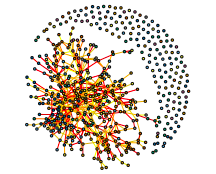
\includegraphics{full_network}
    \caption{Co-authorship network of IITM Professors}
    \label{fig:full_network}
\end{figure}


\section{Data Acquisition}

\begin{figure*}[t]
    \centering
    \includegraphics[width=\textwidth,height=4cm]{CNA_workflow}
    \caption{Program Workflow}
    \label{fig:workflow}
\end{figure*}

In this project, the first step we took was to collect the data for the co-authorship network, which was the list of number of coauthored papers between pairs of professors of IIT Madras. We collected the details of the professors from all the Science-Stream departments(i.e., all departments except Humanities and Management). Publication lists are available at several databases like Google Scholar,DBLP, homepages of authors etc. Since we were interested in the number of co-authored papers only, and not the details of the publication, the data in the above mentioned databases was not in a user-friendly format for our purposes.

The database on Scopus\textsuperscript{\hyperref[sec:thebibliography]{\cite{scopus}}} contained the data in the format we required under the co-authors tab of each author’s profile. We made attempts to use a web-crawler using a Python API\textsuperscript{\hyperref[sec:thebibliography]{\cite{scopus-api}}} to automatically obtain data from the website. However, the authors on Scopus did not have a label to identify them as IIT Madras professors. We then used the faculty list on the institute website \textsuperscript{\hyperref[sec:thebibliography]{\cite{iitm-web}}} to look up the names of the professors and manually extracted the details of the co-authors from their Scopus profile using the API. We then saved the list of coauthors for each author in a separate file. These files were used in the next step where we parsed the data and formed the networks using R\textsuperscript{\hyperref[sec:thebibliography]{\cite{cran-r}}}.

In the data collection process, we have only looked at number of co-authorships between pairs of professors. We haven't looked at publications in which a set of authors have collaborated. 

All the code files for the project and all the plots (some of which haven't been shown in the paper) have been put up in the \href{https://github.com/ashutoshkrjha/EE5154_Repo}{GitHub Repository} of the project.
\section{Network Formation}

Figure \ref{fig:workflow} gives a pictorial representation of the methods we used to process the data and work with the network. After extracting the data about the co-authors of each faculty member, we went about building an adjacency matrix to represent the network. This was done by using our own scripts to parse the csv (comma-separated value) files obtained from Scopus and form an ordered list of all the faculty members of IIT Madras; then, the adjacency matrix was populated using values from the same files that specify which author collaborated with which other author and for how many publications. This adjacency matrix represents an undirected weighted simple network with a node assigned to each individual faculty member and edges with weights corresponding to the number of publications which the two linked faculty members have co-authored. We then used the \emph{igraph}\textsuperscript{\hyperref[sec:thebibliography]{\cite{igraph}}} library in R to visualize the graph and obtain the images shown in this report. We used the packages \emph{igraph}\textsuperscript{\hyperref[sec:thebibliography]{\cite{igraph}}} and \emph{networkx}\textsuperscript{\hyperref[sec:thebibliography]{\cite{networkx}}} for obtaining the performance metrics.




\section{Metrics used for Network Analysis}

We used the following network metrics to analyse our network. This analysis was done across the whole network as well as department-wise.

\noindent \emph{Average Path Length(APL)} : It is equal to the average of the shortest distance between every connected pair of nodes. It is a measure of the mean separation of the nodes in the network. In the presence of disconnected clusters we evaluated the the APL individually for the clusters and then used a weighted average(weighted by the size of the cluster).
Mathematically, we have:
\begin{center}
$\displaystyle{a = \sum\limits_{s,t \in V} \frac{d(s,t)}{n(n-1)}}$
\end{center}
where $V$ is the set of nodes in the network $G$. $d(s,t)$ is the shortest path from $s$ to $t$ and $n$ is the number of nodes in $G$.

\noindent \emph{Diameter(DI)} :  The longest distance between all pairs of nodes. It is a measure of “how far apart is the most distant pair”. Here, in the presence of disconnected clusters, we considered the largest diameter amongst all the circles.

\noindent \emph{Collaborators (CL)}: Average number of collaborators an author has. We find an approximate average clustering coefficient for G by repeating n times (or trials) the following experiment: Choose a node at random, choose two of its neighbors at random, and check if they are connected. The approximate coefficient is the fraction of triangles found over the number of trials. 

\noindent \emph{Clustering Coefficient (CC)}: Clustering co-efficient of the entire network.

\noindent \emph{Largest component (LC):} The number of the nodes that are present in the largest connected component of the network.

\section{Observations}

The following observations were made by using visualisations of the networks

\subsubsection*{Intra-Departmental Connections}


EE(Figure \ref{fig:ee}) and EP(Figure \ref{fig:ep}) department networks appear to be the most well connected networks.These networks have a single well branched chain. CE has two chains of appreciable lengths which are not connected(as seen in Figure \ref{fig:civil}). CH(Figure \ref{fig:ch}) graph indicates that in the connected chain many pairs of nodes are connected by multiple edges indicating that the links are strong (weights are represented by number of edges). Chemistry graph features small well connected groups.

\begin{figure}[t]
    \centering
    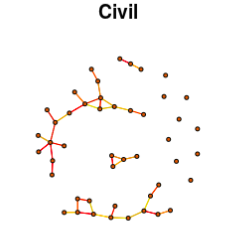
\includegraphics[width=5cm,height=5cm]{civil}
    \caption{Co-authorship network in Dept. of Civil Engineering}
    \label{fig:civil}
\end{figure}

A general theme among all the department graphs is that there are tightly knit groups, or often cliques of size 3. Also, a large number of isolated vertices exist in each department’s network. If we analyze any clique, we note that the collaborating professors often work in the same group within the department, for example Dr. Sarit K. Das and Dr.Sundararajan,T. have a lot of collaborations and also happen to be working in the same research group in the Thermal Power Engineering Lab in the Mechanical Engineering Department. This close knit structure is in accordance with the trend in other social networks where people who have a lot in common often form cliques in such networks.

\subsubsection*{Inter-Departmental Connections}

The inter department connections are uniformly present among the departments(as seen in Figure \ref{fig:interdept},also see Table \ref{tab:inter-dep}). Each department has a degree of around 9-11 barring the Mathematics department. It has to be however noted that the number of co-authored documents in inter-disciplinary research is significantly lower as compared to the total number of co-authored documents published within a department.Also, we can see that there are pairs of departments which have a relatively high number of collaborations, for example ME and CH, and MM and PH, and EE and CS. This is as expected because these pairs of departments have a significant overlap in the fields which they study. Hence, this is not complete evidence that there is interdisciplinary research being conducted. 

\begin{figure}[t]
    \centering
    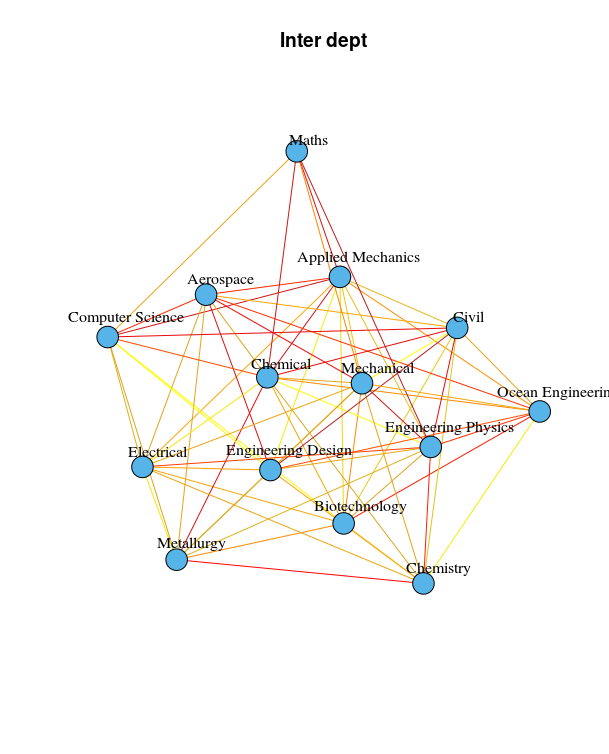
\includegraphics[width=6cm,height=8cm]{inter_dept}
    \caption{Co-authorship between departments}
    \label{fig:interdept}
\end{figure}

\subsubsection*{Network Attributes}

Network attributes were calculated department-wise using igraph and networkx packages. The attribute values have been recorded in Table \ref{tab:net_attri}. 

\begin{table}[h]
\centering
\caption{Department-wise Network Parameters}
\label{tab:net_attri}
\begin{tabular}{|l|l|l|l|l|}
\hline
            & \textbf{APL} & \textbf{DI} & \textbf{CC} & \textbf{LC} \\ \hline
\textbf{CH} & 3.142        & 7           & 0.120       & 21          \\ \hline
\textbf{CE} & 3.616        & 9           & 0.079       & 18          \\ \hline
\textbf{ED} & 1.285        & 2           & 0.0         & 4           \\ \hline
\textbf{EE} & 3.979        & 10          & 0.142       & 45          \\ \hline
\textbf{AE} & 2.531        & 5           & 0.0         & 10          \\ \hline
\textbf{AM} & 1.25         & 2           & 0.0         & 3           \\ \hline
\textbf{BT} & 2.890        & 6           & 0.170       & 13          \\ \hline
\textbf{CS} & 2.361        & 4           & 0.0         & 12          \\ \hline
\textbf{ME} & 3.662        & 8           & 0.076       & 34          \\ \hline
\textbf{MM} & 2.388        & 5           & 0.096       & 12          \\ \hline
\textbf{OE} & 2.839        & 6           & 0.269       & 17          \\ \hline
\textbf{CY} & 2.425        & 5           & 0.057       & 9           \\ \hline
\textbf{PH} & 3.197        & 8           & 0.058       & 34          \\ \hline
\textbf{MA} & 1.461        & 2           & 0.0         & 5           \\ \hline
\textbf{All} & \textbf{5.505}        & \textbf{14}           & \textbf{0.011}         & \textbf{193}           \\ \hline
\end{tabular}
\end{table}

\subsubsection*{Department Leaders}

The following professors were found to have the most number of collaborations: 
\begin{itemize}
\item Sayan Gupta(AM)
\item Vignesh Muthuvijayan(BT)
\item Manikandan Mathur(AE)
\item Raghunathan  Rengasamy(CH)
\item Ashok Kumar Mishra(CY)
\item Ramaswamy Sivanandan(CE)
\item S.Ganesh Sundara Raman(MM)
\item Veezhinathan  Kamakoti(CS)
\item Venkatesh Balasubramanian(ED)
\item Shanthi  Pavan(EE)
\item Ashwin Joy(EP)
\item Raghavan Rama(MA)
\item Ravikiran  Sangras(ME)
\item Govindarajan SureshKumar(OE)
\end{itemize}

\subsubsection*{Similarity to a Social Network:}
In trying to analyse the Co-authorship network as a Social Network, we can draw an analogy to a Network of Friends. Authors could be analogous to people,collaborations to friends(and hence the strength of the friendship is signified by the number of collaborations),departments to cities, cliques to a friend-circle(each person knows the other) and a chain of collaborations to a chain of friends. Using this analogy we can see the remarkable resemblance of our network to a Social Network.

We see that most collaborations happen within the department(friendships within the city). Even in those inter-departmental collaborations that do exist, the number of collaborations seems to be low(just like friendships across city). There are many more such comparisons that can be done. 



% An example of a floating figure using the graphicx package.
% Note that \label must occur AFTER (or within) \caption.
% For figures, \caption should occur after the \includegraphics.
% Note that IEEEtran v1.7 and later has special internal code that
% is designed to preserve the operation of \label within \caption
% even when the captionsoff option is in effect. However, because
% of issues like this, it may be the safest practice to put all your
% \label just after \caption rather than within \caption{}.
%
% Reminder: the "draftcls" or "draftclsnofoot", not "draft", class
% option should be used if it is desired that the figures are to be
% displayed while in draft mode.
%
%\begin{figure}[!t]
%\centering
%\includegraphics[width=2.5in]{myfigure}
% where an .eps filename suffix will be assumed under latex, 
% and a .pdf suffix will be assumed for pdflatex; or what has been declared
% via \DeclareGraphicsExtensions.
%\caption{Simulation results for the network.}
%\label{fig_sim}
%\end{figure}

% Note that the IEEE typically puts floats only at the top, even when this
% results in a large percentage of a column being occupied by floats.


% An example of a double column floating figure using two subfigures.
% (The subfig.sty package must be loaded for this to work.)
% The subfigure \label commands are set within each subfloat command,
% and the \label for the overall figure must come after \caption.
% \hfil is used as a separator to get equal spacing.
% Watch out that the combined width of all the subfigures on a 
% line do not exceed the text width or a line break will occur.
%
%\begin{figure*}[!t]
%\centering
%\subfloat[Case I]{\includegraphics[width=2.5in]{box}%
%\label{fig_first_case}}
%\hfil
%\subfloat[Case II]{\includegraphics[width=2.5in]{box}%
%\label{fig_second_case}}
%\caption{Simulation results for the network.}
%\label{fig_sim}
%\end{figure*}
%
% Note that often IEEE papers with subfigures do not employ subfigure
% captions (using the optional argument to \subfloat[]), but instead will
% reference/describe all of them (a), (b), etc., within the main caption.
% Be aware that for subfig.sty to generate the (a), (b), etc., subfigure
% labels, the optional argument to \subfloat must be present. If a
% subcaption is not desired, just leave its contents blank,
% e.g., \subfloat[].


% An example of a floating table. Note that, for IEEE style tables, the
% \caption command should come BEFORE the table and, given that table
% captions serve much like titles, are usually capitalized except for words
% such as a, an, and, as, at, but, by, for, in, nor, of, on, or, the, to
% and up, which are usually not capitalized unless they are the first or
% last word of the caption. Table text will default to \footnotesize as
% the IEEE normally uses this smaller font for tables.
% The \label must come after \caption as always.
%
%\begin{table}[!t]
%% increase table row spacing, adjust to taste
%\renewcommand{\arraystretch}{1.3}
% if using array.sty, it might be a good idea to tweak the value of
% \extrarowheight as needed to properly center the text within the cells
%\caption{An Example of a Table}
%\label{table_example}
%\centering
%% Some packages, such as MDW tools, offer better commands for making tables
%% than the plain LaTeX2e tabular which is used here.
%\begin{tabular}{|c||c|}
%\hline
%One & Two\\
%\hline
%Three & Four\\
%\hline
%\end{tabular}
%\end{table}


% Note that the IEEE does not put floats in the very first column
% - or typically anywhere on the first page for that matter. Also,
% in-text middle ("here") positioning is typically not used, but it
% is allowed and encouraged for Computer Society conferences (but
% not Computer Society journals). Most IEEE journals/conferences use
% top floats exclusively. 
% Note that, LaTeX2e, unlike IEEE journals/conferences, places
% footnotes above bottom floats. This can be corrected via the
% \fnbelowfloat command of the stfloats package.




\section{Conclusion}
In this paper we analysed the co-authorship network in IIT Madras. We provided visualisations of the entire network as well as the intra- and inter-department networks. Also, we also measured a few vital network parameters in the department networks. As expected, the intra-departmental collaborations were more than that of inter-departmental collaborations. Again, as expected but less obvious, even within departments we saw formation of clusters of authors which in many cases corresponded to fields of study within the department.

This study has given us considerable insights into the nature of collaborations among the professors in the institute. The network throws light on the nature of intra- and inter-departmental research(or the lack of?) happening in the institute. This could help the institute plan its future research endeavours in the direction of inter-disciplinary research.


\section{Future Work}
We see two ways of expanding on the project in the future:
\begin{itemize}
\item We could expand the analysis to multiple institutes and even look at inter-institute collaborations. In this paper we have only considered the professors' collaboration in our analysis. We could also extend this to the students and other researchers in the institute.
\item In this paper we have constructed the network using only the number of co-authorships as the data. In the future, we could also look at papers in which a set of professors have collaborated. We could then construct hyper-graphs which would contain much more information.  
\end{itemize}



% conference papers do not normally have an appendix



% use section* for acknowledgment
\ifCLASSOPTIONcompsoc
  % The Computer Society usually uses the plural form
  \section*{Acknowledgments}
\else
  % regular IEEE prefers the singular form
  \section*{Acknowledgment}
\fi


The authors would like to thank Dr. Venkatesh Ramaiyan for having given them an opportunity to work on this project, and also for providing references and guidance during the project.





% trigger a \newpage just before the given reference
% number - used to balance the columns on the last page
% adjust value as needed - may need to be readjusted if
% the document is modified later
%\IEEEtriggeratref{8}
% The "triggered" command can be changed if desired:
%\IEEEtriggercmd{\enlargethispage{-5in}}

% references section

% can use a bibliography generated by BibTeX as a .bbl file
% BibTeX documentation can be easily obtained at:
% http://mirror.ctan.org/biblio/bibtex/contrib/doc/
% The IEEEtran BibTeX style support page is at:
% http://www.michaelshell.org/tex/ieeetran/bibtex/
%\bibliographystyle{IEEEtran}
% argument is your BibTeX string definitions and bibliography database(s)
%\bibliography{IEEEabrv,../bib/paper}
%
% <OR> manually copy in the resultant .bbl file
% set second argument of \begin to the number of references
% (used to reserve space for the reference number labels box)
\begin{thebibliography}{1}

\bibitem{holland} P. W. Holland and S. Leinhardt (1971). "Transitivity in structural models of small groups". Comparative Group Studies. 2: 107–124.

\bibitem{watts}  D. J. Watts and Steven Strogatz (June 1998). "Collective dynamics of 'small-world' networks". Nature. 393 (6684): 440–442.

\bibitem{tasleem} Tasleem Arif, Rashid Ali, M.Asger (August 2012). "Scientific Co-authorship Social Networks: A Case Study of Computer Science Scenario in India".International Journal of Computer Applications (0975 – 8887) Volume 52– No.12

\bibitem{scopus} \href{https://www.scopus.com/home.uri}{Scopus | The largest database of peer-reviewed literature | Elsevier}

\bibitem{scopus-api} \href{https://github.com/jkitchin/scopus}{John R. Kitchin: Python API for Accessing Scopus databases with their REST API}

\bibitem{iitm-web} \href{https://www.iitm.ac.in/}{Indian Institute of Technology Madras: Official Website}

\bibitem{cran-r} \href{https://cran.r-project.org/}{The Comprehensive R Archive Network}

\bibitem{igraph} \href{http://igraph.org/python/}{python-igraph}

\bibitem{networkx} \href{https://networkx.github.io/}{NetworkX-Python}

\bibitem{networkx}
\href{https://github.com/ashutoshkrjha/EE5154_Repo}{GitHub Repository of the Project}
\end{thebibliography}

\section*{Appendix-A}

\subsubsection*{Inter-Department Collabration Matrix:} 
In Table \ref{tab:inter-dep}, we have recorded the number of inter-department collaborations among different departments. We have set the intra-department count to 0 as that has been studied extensively in the rest of the paper.
\begin{table}[h]
\centering
\caption{Number of Interdepartment collaborations}
\label{tab:inter-dep}
\resizebox{\columnwidth}{!}{%
\begin{tabular}{|l|l|l|l|l|l|l|l|l|l|l|l|l|l|l|}
\hline
\textbf{}    & \textbf{AM} & \textbf{BT} & \textbf{AE} & \textbf{CH} & \textbf{CY} & \textbf{CE} & \textbf{CSE} & \textbf{ED} & \textbf{EE} & \textbf{PH} & \textbf{MA} & \textbf{ME} & \textbf{MM} & \textbf{OE} \\ \hline
\textbf{AM}  & 0           & 4           & 6           & 2           & 0           & 10          & 1            & 9           & 1           & 3           & 2           & 14          & 0           & 3           \\ \hline
\textbf{BT}  & 4           & 0           & 0           & 6           & 11          & 8           & 6            & 0           & 4           & 6           & 0           & 4           & 17          & 9           \\ \hline
\textbf{AE}  & 6           & 0           & 0           & 5           & 0           & 1           & 1            & 3           & 11          & 0           & 0           & 26          & 7           & 6           \\ \hline
\textbf{CH}  & 2           & 6           & 5           & 0           & 5           & 6           & 1            & 0           & 4           & 9           & 7           & 33          & 13          & 1           \\ \hline
\textbf{CY}  & 0           & 11          & 0           & 5           & 0           & 5           & 0            & 1           & 6           & 23          & 0           & 23          & 4           & 16          \\ \hline
\textbf{CE}  & 10          & 8           & 1           & 6           & 5           & 0           & 4            & 3           & 0           & 9           & 0           & 9           & 0           & 8           \\ \hline
\textbf{CSE} & 1           & 6           & 1           & 1           & 0           & 4           & 0            & 2           & 24          & 0           & 1           & 0           & 1           & 0           \\ \hline
\textbf{ED}  & 9           & 0           & 3           & 0           & 1           & 3           & 2            & 0           & 17          & 2           & 0           & 8           & 2           & 3           \\ \hline
\textbf{EE}  & 1           & 4           & 11          & 4           & 6           & 0           & 24           & 17          & 0           & 18          & 0           & 12          & 12          & 0           \\ \hline
\textbf{PH}  & 3           & 6           & 0           & 9           & 23          & 9           & 0            & 2           & 18          & 0           & 3           & 28          & 51          & 2           \\ \hline
\textbf{MA}  & 2           & 0           & 0           & 7           & 0           & 0           & 1            & 0           & 0           & 3           & 0           & 2           & 0           & 0           \\ \hline
\textbf{ME}  & 14          & 4           & 26          & 33          & 23          & 9           & 0            & 8           & 12          & 28          & 2           & 0           & 23          & 2           \\ \hline
\textbf{MM}  & 0           & 17          & 7           & 13          & 4           & 0           & 1            & 2           & 12          & 51          & 0           & 23          & 0           & 0           \\ \hline
\textbf{OE}  & 3           & 9           & 6           & 1           & 16          & 8           & 0            & 3           & 0           & 2           & 0           & 2           & 0           & 0           \\ \hline
\end{tabular}%
}
\end{table}

\newpage

\subsubsection*{Intra-Department Plots:}

Following are the plots of a selected number of departments. For a collection of all the plots please refer to the \href{https://github.com/ashutoshkrjha/EE5154_Repo}{GitHub Repository} of the project.

\begin{figure}[h]
    \centering
    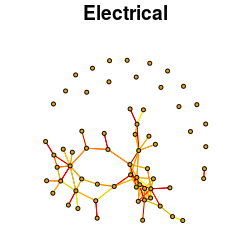
\includegraphics[width=5cm,height=5cm]{ee}
    \caption{Co-authorship network in Dept. of Electrical Engineering}
    \label{fig:ee}
\end{figure}

\begin{figure}[h]
    \centering
    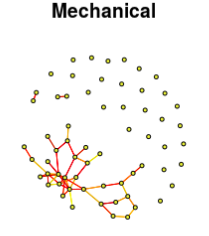
\includegraphics[width=5cm,height=5cm]{me}
    \caption{Co-authorship network in Dept. of Mechanical Engineering}
    \label{fig:me}
\end{figure}

\begin{figure}[h]
    \centering
    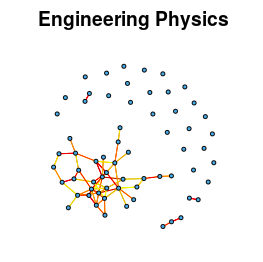
\includegraphics[width=5cm,height=5cm]{ep}
    \caption{Co-authorship network in Dept. of Physics}
    \label{fig:ep}
\end{figure}

\begin{figure}[t]
    \centering
    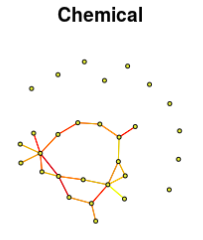
\includegraphics[width=5cm,height=5cm]{ch}
    \caption{Co-authorship network in Dept. of Chemical Engineering}
    \label{fig:ch}
\end{figure}


% that's all folks
\end{document}


